\subsection{Elemek elhelyezése}

%_
\begin{frame}
  \begin{columns}[c]
    \column{0.5\textwidth}
      A \texttt{position} tulajdonsággal befolyásolható az elemek elhelyezési módja az oldalon. Értékei:
      \begin{description}[m]
        \item[\texttt{static}] \hfill \\ Alapértelmezett elrendezés. A böngésző dönt az elemek helyéről és ált. a méretezéséről is (pl. blokkszintű elemek egymás alatt/egymáson belül, széltében kitöltik a rendelkezésre álló helyet, soron belüliek a blokkszintűek belsejében, stb.)
      \end{description}
    \column{0.45\textwidth}
      \begin{exampleblock}{\textattachfile{static.html}{static.html}}
        \scriptsize
        \lstinputlisting[style=HTML,linerange={7-12},numbers=right,firstnumber=7]{static.html}
        \lstinputlisting[style=HTML,linerange={16-18},numbers=right,firstnumber=16]{static.html}
      \end{exampleblock}
      \begin{center}
        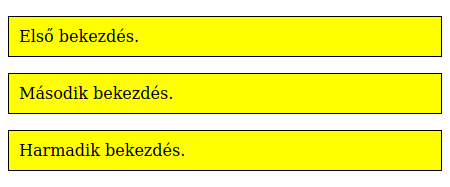
\includegraphics[width=0.5\textwidth]{static.png}
      \end{center}
  \end{columns}
\end{frame}

%_
\begin{frame}
  \begin{columns}[T]
    \column{0.35\textwidth}
      \begin{description}[m]
        \item[\texttt{relative}] \hfill \\ Az elem az eredeti helyéhez képest eltolható, de ezt a régi helyet a böngésző fenntartja. Megadható az elem tetejének (\texttt{top}), aljának (\texttt{bottom}), bal (\texttt{left}) és jobb oldalának (\texttt{right}) relatív helyzete.
      \end{description}
      \vfill
      \begin{center}
        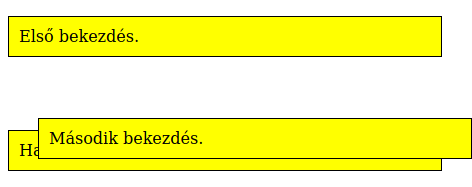
\includegraphics[width=.75\textwidth]{relative.png}
      \end{center}
    \column{0.6\textwidth}
      \begin{exampleblock}{\textattachfile{relative.html}{relative.html}}
        \scriptsize
        \lstinputlisting[style=HTML,linerange={7-16},numbers=right,firstnumber=7]{relative.html}
        \lstinputlisting[style=HTML,linerange={20-22},numbers=right,firstnumber=20]{relative.html}
      \end{exampleblock}
  \end{columns}
\end{frame}

%_
\begin{frame}
  \begin{description}[m]
    \item[\texttt{absolute}] \hfill \\ A legközelebbi, nem statikusan elhelyezett szülő elemhez, annak hiányában a dokumentum testéhez képest relatívan megadott helyre igazítja az elemet. Az elem eredeti helyét nem őrzi meg a böngésző.
  \end{description}
  \vfill
  \begin{center}
    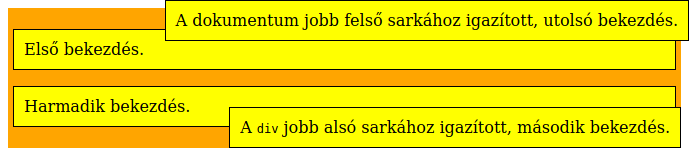
\includegraphics[width=.6\textwidth]{absolute.png}\\
    \textattachfile{absolute.html}{absolute.html}
  \end{center}
\end{frame}

%_
\begin{frame}
  \begin{columns}[c]
    \column{0.45\textwidth}
      \begin{exampleblock}{\textattachfile{absolute.html}{absolute.html}}
        \fontsize{7}{8} \selectfont
        \lstinputlisting[style=HTML,linerange={7-22},numbers=left,firstnumber=7]{absolute.html}
      \end{exampleblock}
    \column{0.5\textwidth}
      \begin{exampleblock}{}
        \fontsize{7}{8} \selectfont
        \lstinputlisting[style=HTML,linerange={23-28},numbers=right,firstnumber=23]{absolute.html}
        \lstinputlisting[style=HTML,linerange={32-41},numbers=right,firstnumber=32]{absolute.html}
      \end{exampleblock}
  \end{columns}
\end{frame}

%_
\begin{frame}
  \begin{description}[m]
    \item[\texttt{fixed}] \hfill \\ Az elem pozíciója a nézetablakhoz képest relatív, görgetés közben is a helyén marad.
  \end{description}
  \begin{columns}[c]
    \column{0.45\textwidth}
      \begin{center}
        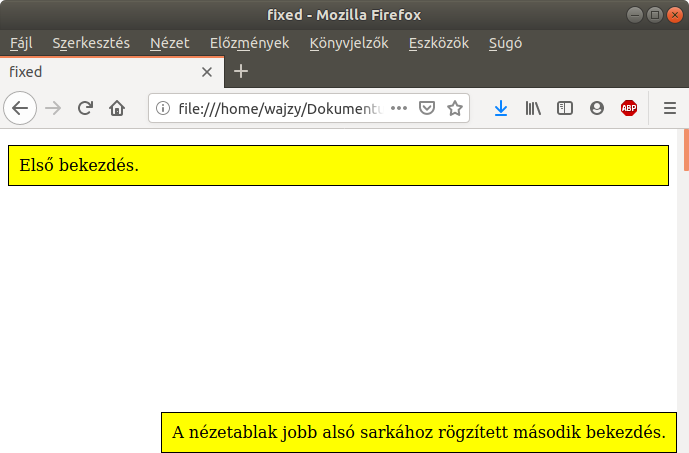
\includegraphics[width=\textwidth]{fixed1.png}
      \end{center}
    \column{0.45\textwidth}
      \begin{center}
        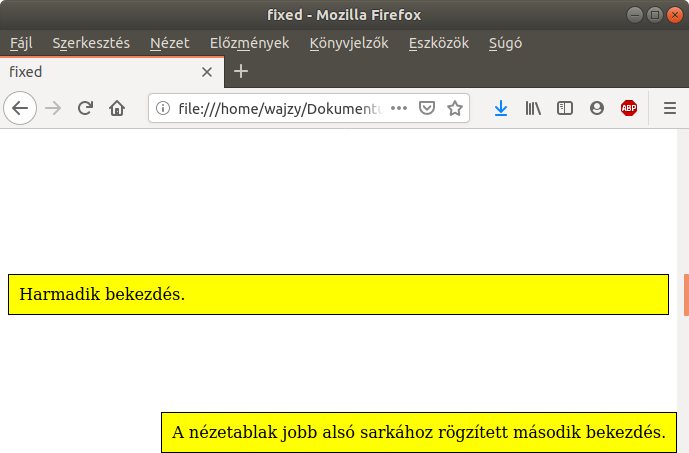
\includegraphics[width=\textwidth]{fixed2.png}
      \end{center}
  \end{columns}
  \begin{center}
    \textattachfile{fixed.html}{fixed.html} -- Figyeljék a gördítősávot!
  \end{center}
\end{frame}

%_
\begin{frame}
  \begin{columns}[T]
    \column{0.43\textwidth}
      \begin{exampleblock}{\textattachfile{fixed.html}{fixed.html}}
        \scriptsize
        \lstinputlisting[style=HTML,linerange={7-18},numbers=left,firstnumber=7]{fixed.html}
      \end{exampleblock}
    \column{0.53\textwidth}
      \begin{exampleblock}{}
        \scriptsize
        \lstinputlisting[style=HTML,linerange={22-26},numbers=right,firstnumber=22]{fixed.html}
      \end{exampleblock}
  \end{columns}  
\end{frame}

%_
\begin{frame}
  \begin{description}[m]
    \item[\texttt{sticky}] \hfill \\ A \texttt{relative} és a \texttt{fixed} kombinációja; az elem gördül a nézetablak tartalmával, amíg el nem ér egy adott helyre, ahová ,,odaragad''.\\
    \vspace{0.3cm} \tiny Részleges böngésző támogatás; pl. Safarin a \texttt{-webkit-sticky} értékkel működik csak.
  \end{description}
  \begin{columns}[T]
    \column{0.3\textwidth}
      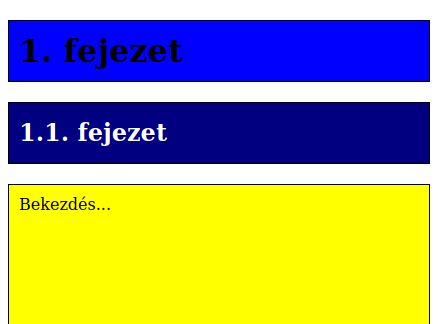
\includegraphics[width=\textwidth]{sticky1.png}
    \column{0.3\textwidth}
      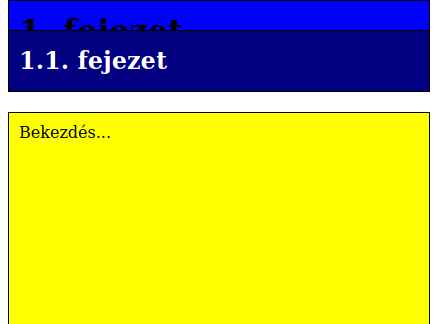
\includegraphics[width=\textwidth]{sticky2.png}
    \column{0.3\textwidth}
      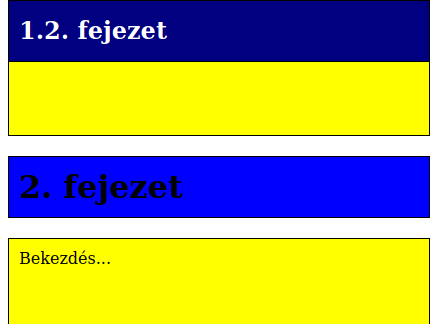
\includegraphics[width=\textwidth]{sticky3.png}
  \end{columns}
  \begin{center}
    \textattachfile{sticky.html}{sticky.html} -- Próbálják görgetni a tartalmat!
  \end{center}
\end{frame}

%_
\begin{frame}
  \begin{columns}[c]
    \column{0.45\textwidth}
      \begin{exampleblock}{\textattachfile{sticky.html}{sticky.html}}
        \fontsize{7}{8} \selectfont
        \lstinputlisting[style=HTML,linerange={7-23},numbers=left,firstnumber=7]{sticky.html}
      \end{exampleblock}
    \column{0.5\textwidth}
      \begin{exampleblock}{}
        \fontsize{7}{8} \selectfont
        \lstinputlisting[style=HTML,linerange={24-29},numbers=right,firstnumber=24]{sticky.html}
        \lstinputlisting[style=HTML,linerange={33-39},numbers=right,firstnumber=33]{sticky.html}
      \end{exampleblock}
  \end{columns}
\end{frame}

%_
\begin{frame}
  Próbálja meg elkészíteni az alábbi \textattachfile{gabor.html}{weboldalt} a \textattachfile{gabor.txt}{gabor.txt} és \textattachfile{gabor.jpeg}{gabor.jpeg} fájlok felhasználásával!
  \vfill
  \begin{columns}[T]
    \column{0.3\textwidth}
      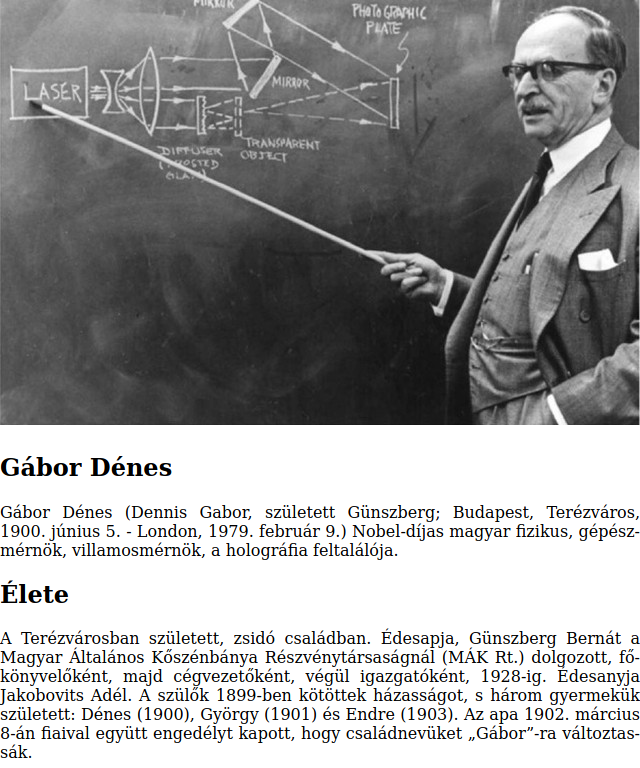
\includegraphics[width=\textwidth]{gabor1.png}
    \column{0.3\textwidth}
      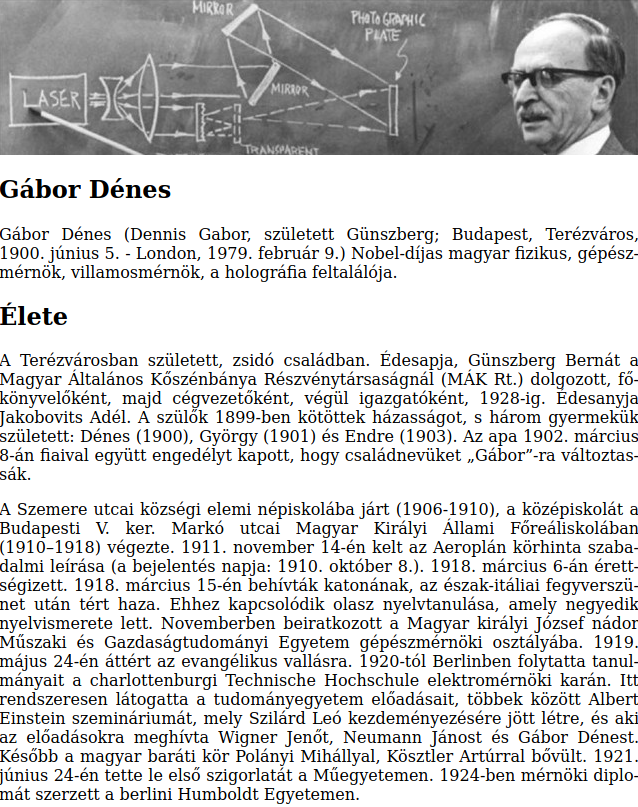
\includegraphics[width=\textwidth]{gabor2.png}
    \column{0.3\textwidth}
      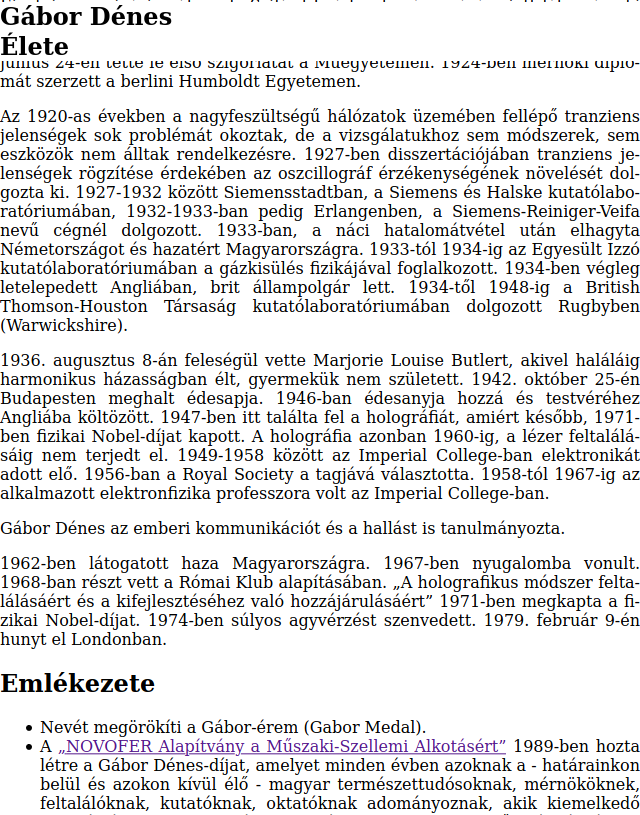
\includegraphics[width=\textwidth]{gabor3.png}
  \end{columns}
\end{frame}

%_
\begin{frame}
  Az oldal elvárt viselkedése a következő:
  \begin{itemize}
    \item A kép egyhelyben áll a görgetés hatására is. A felfelé gördülő szöveg lassan rácsúszik, majd teljesen kitakarja azt.
    \item Az első szintű címsor addig csúszik felfelé, amíg el nem éri a nézetablak tetejét. Utána ottmarad, és a bekezdések szövege alágördül.
    \item A második szintű címsor hasonlóan viselkedik az első szintűhöz, de az alatt áll meg, nem takarja le azt. A második szintű címsorok viszont letakarhatják egymást.
    \item A cikk maximális szélessége 640 képpont. Ha ennél több hely áll rendelkezésre, középre kell igazítani.
    \item A szöveg sorkizárt igazítású, automatikusan elválasztott.
    \item Az idézetek előtt és után magyar stílusú (,, '') idézőjeleket alkalmaz.
    \item A hivatkozás új oldalon nyílik meg.
  \end{itemize}
\end{frame}
